\documentclass{beamer}[10]

\usepackage{graphicx}
\usepackage{xcolor}
\usepackage{tabto}
%\usepackage{beamerthemesplit}
\usepackage{tikz}
\usepackage{cancel}
\usepackage{verbatim}
\usepackage{fancybox}
\usepackage{enumerate}
\usepackage{amsmath,amssymb,amsthm,textcomp,mathtools}
\usepackage[super]{nth}
\usepackage[amssymb]{SIunits}
\usepackage{booktabs}
\usepackage{cancel}
\usepackage{bm}
\usepackage[utf8]{inputenc}
\usepackage{tabularx}
\usepackage{ragged2e}
\newcolumntype{Y}{ >{\RaggedRight\arraybackslash}X}
\usetikzlibrary{arrows,shapes}
\newcommand\T{\rule{0pt}{2.6ex}}
\newcommand\B{\rule[-1.2ex]{0pt}{0pt}}
\definecolor{UUcrimson}{RGB}{204,0,0}
\mode<presentation>
{ \usetheme{default}
  \usecolortheme[named=UUcrimson]{structure}
  \useinnertheme{circles}
  \setbeamercovered{transparent}
  \setbeamertemplate{blocks}[rounded]
  \usefonttheme[onlymath]{serif}
  \setbeamertemplate{navigation symbols}{}
  \setbeamertemplate{footline}[page number]
  \setbeamertemplate{navigation symbols}{}
  \setbeamercolor{section in toc}{fg=black,bg=white}
  \setbeamercolor{alerted text}{fg=UUcrimson!80!gray}
  \setbeamercolor*{palette primary}{fg=white,bg=UUcrimson}
  \setbeamercolor*{palette secondary}{fg=UUcrimson!70!black,bg=gray!15!white}
  \setbeamercolor*{palette tertiary}{bg=UUcrimson!80!black,fg=gray!10!white}
  \setbeamercolor*{palette quaternary}{fg=UUcrimson,bg=gray!5!white}
  \setbeamercolor*{palette sidebar primary}{fg=UUcrimson!10!black}
  \setbeamercolor*{palette sidebar secondary}{fg=white}
  \setbeamercolor*{palette sidebar tertiary}{fg=UUcrimson!50!black}
  \setbeamercolor*{palette sidebar quaternary}{fg=gray!10!white}
  \setbeamercolor{titlelike}{parent=palette primary,fg=white}
  \setbeamercolor{frametitle}{bg=UUcrimson}
  \setbeamercolor{frametitle right}{bg=UUcrimson}
  \setbeamercolor*{separation line}{}
  \setbeamercolor*{fine separation line}{}
}

\usetikzlibrary{backgrounds}
\makeatletter
\tikzstyle{every picture}+=[remember picture]
\tikzset{%
  fancy quotes/.style={
    text width=\fq@width pt,
    align=justify,
    inner sep=1em,
    anchor=north west,
    minimum width=\linewidth,
    font=\itshape
  },
  fancy quotes width/.initial={.8\linewidth},
  fancy quotes marks/.style={
    scale=8,
    text=white,
    inner sep=0pt,
  },
  fancy quotes opening/.style={
    fancy quotes marks,
  },
  fancy quotes closing/.style={
    fancy quotes marks,
  },
  fancy quotes background/.style={
    show background rectangle,
    inner frame xsep=0pt,
    background rectangle/.style={
      fill=gray!25,
      rounded corners,
    },
  }
}
\newenvironment{fancyquotes}[1][]{%
\noindent
\tikzpicture[fancy quotes background]
\node[fancy quotes opening,anchor=north west] (fq@ul) at (0,0) {``};
\tikz@scan@one@point\pgfutil@firstofone(fq@ul.east)
\pgfmathsetmacro{\fq@width}{\linewidth - 2*\pgf@x}
\node[fancy quotes,#1] (fq@txt) at (fq@ul.north west) \bgroup}
{\egroup;
\node[overlay,fancy quotes closing,anchor=east] at (fq@txt.south east) {''};
\endtikzpicture}
\makeatother


\usetikzlibrary{backgrounds}
\makeatletter
\tikzstyle{every picture}+=[remember picture]
\tikzset{%
  fancy defs/.style={
    text width=\fq@width pt,
    align=justify,
    inner sep=0.25em,
    anchor=north west,
    minimum width=\linewidth,
    font=\itshape
  },
  fancy defs width/.initial={.8\linewidth},
  fancy defs marks/.style={
    scale=8,
    text=white,
    inner sep=0pt,
  },
  fancy defs opening/.style={
    fancy defs marks,
  },
  fancy defs closing/.style={
    fancy defs marks,
  },
  fancy defs background/.style={
    show background rectangle,
    inner frame xsep=0pt,
    background rectangle/.style={
      fill=gray!25,
      rounded corners,
    },
  }
}
\newenvironment{fancydefs}[1][]{%
\noindent
\tikzpicture[fancy defs background]
\node[fancy defs opening,anchor=north west] (fq@ul) at (0,0) {};
\tikz@scan@one@point\pgfutil@firstofone(fq@ul.east)
\pgfmathsetmacro{\fq@width}{\linewidth - 2*\pgf@x}
\node[fancy defs,#1] (fq@txt) at (fq@ul.north west) \bgroup}
{\egroup;
\node[overlay,fancy defs closing,anchor=east] at (fq@txt.south east) {};
\endtikzpicture}
\makeatother
\usepackage{scalerel}[2014/03/10]
\usepackage{stackengine}
\usepackage{empheq}
\newcommand*\widefbox[1]{\fbox{\hspace{0.5em}#1\hspace{0.5em}}}

\newcommand\reallywidetilde[1]{\ThisStyle{%
  \setbox0=\hbox{$\SavedStyle#1$}%
  \stackengine{-.1\LMpt}{$\SavedStyle#1$}{%
    \stretchto{\scaleto{\SavedStyle\mkern.2mu\sim}{.5467\wd0}}{.4\ht0}%
%    .2mu is the kern imbalance when clipping white space
%    .5467++++ is \ht/[kerned \wd] aspect ratio for \sim glyph
  }{O}{c}{F}{T}{S}%
}}
\usepackage{media9}

\logo{
\includegraphics[width=0.75cm]{logo.jpg}}
\author[Gibbs]{Dr. Jeremy A. Gibbs}
\institute{Department of Mechanical Engineering\\University of Utah}
\date{Spring 2017}
\title{Environmental Fluid Dynamics: Lecture 12}
% colors
\newcommand{\ihat}{\boldsymbol{\hat{\imath}}}
\newcommand{\jhat}{\boldsymbol{\hat{\jmath}}}
\newcommand{\khat}{\boldsymbol{\hat{k}}}
\definecolor{colororange}{HTML}{E65100} % orange
\definecolor{colordgray}{HTML}{795548} % dark gray for note
\definecolor{colorhgray}{HTML}{212121} % heavy dark gray for normal text
\definecolor{colorgreen}{HTML}{009688} % green
\definecolor{colorwhite}{HTML}{FFFFFF} % background white
\definecolor{colorlgray}{HTML}{F5F3EE} % background light gray
\definecolor{colorblue}{HTML}{0277BB} % blue
\definecolor{colorred}{HTML}{CC0000} % red
\newcommand{\fontsizeone}{1.9em}
\usepackage{esvect}
\setbeamertemplate{caption}{\raggedright\insertcaption\par}
\newcommand{\framecard}[2][colorgreen]{
  {\setbeamercolor{background canvas}{bg=#1}
    \begin{frame}[plain]
    \vfill
    \begin{center}
     {#2}
    \end{center}
    \vfill
    \end{frame}
  }
}
\begin{document}

%----------------------------------------------------------------------------------------
%	TITLE & TOC SLIDES
%----------------------------------------------------------------------------------------

\begin{frame} 
  \titlepage
\end{frame}

%------------------------------------------------

\begin{frame}
\frametitle{Overview}
\tableofcontents
\end{frame}

%------------------------------------------------
\section{The Ekman Layer} %
%------------------------------------------------
\framecard[colorred]{{\color{white}\Huge The Ekman Layer}}
%------------------------------------------------
\subsection{Overview}
\begin{frame}{The Ekman Layer}

Consider a scenario where fluid flow:
\begin{itemize}
	\item is bounded below by a flat boundary,
	\item is purely geostrophic far above this boundary,
	\item is incompressible,
	\item is in a steady state,
	\item has constant density, and
	\item has constant Coriolis (latitude is taken as constant)
\end{itemize}
\end{frame}

%------------------------------------------------
\begin{frame}{The Ekman Layer}

\begin{itemize}
	\item We want to derive an exact solution of the Navier-Stokes equations for this scenario.
	\item We anticipate that this flow behaves as:
	\begin{itemize}
		\item $u(x,y,z,t) = u(z)$
		\item $v(x,y,z,t) = v(z)$
		\item $w(x,y,z,t) = 0$
	\end{itemize}
	\item That is, the flow is in a steady state, has no vertical motion, and is horizontally-uniform in any horizontal plane.
\end{itemize}
\end{frame}

%------------------------------------------------

\subsection{Boundary Conditions}

\begin{frame}{The Ekman Layer: Boundary Conditions}

\textbf{Lower Boundary Conditions}
\begin{itemize}
	\item The ground ($z=0$) is impermeable ($w=0$), which is automatically satisfied since $w$ is assumed to be zero everywhere.
	\item Since this is a viscous flow, we must impose the no-slip condition at the surface [$u(0) = 0, v(0)=0$].
\end{itemize}

\textbf{Upper Boundary Conditions}
\begin{itemize}
	\item The scenario says that the flow is purely geostrophic far away from the lower boundary [$u(\infty)=u_g$, $v(\infty)=v_g$], where the geostrophic components are given by:
	$$-fv_g = -\frac{1}{\rho} \frac{\partial p}{\partial x}(\infty) \qquad fu_g = -\frac{1}{\rho} \frac{\partial p}{\partial y}(\infty)$$
\end{itemize}
\end{frame}

%------------------------------------------------
\subsection{Rotated Coordinate System}

\begin{frame}{The Ekman Layer: Rotated Coordinate System}

\begin{itemize}
	\item We can make life easier if we consider a new Cartesian coordinate system where the $x$-axis is aligned in the direction of the geostrophic wind vector.
	\item Thus, the $y$-axis points int he direction of $-\vv{\nabla}p$ (toward low pressure).
	\begin{align*}
		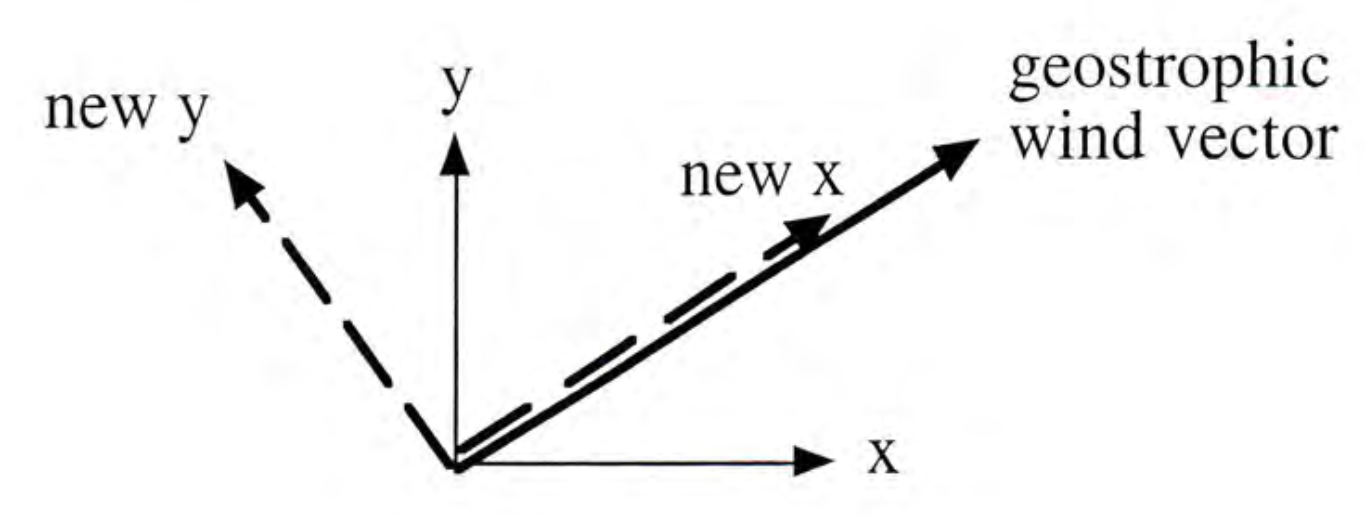
\includegraphics[width=0.8\textwidth]{ekman1}	
	\end{align*}
\end{itemize}
\end{frame}

%------------------------------------------------
\begin{frame}{The Ekman Layer: Rotated Coordinate System}

\begin{itemize}
	\item In this new coordinate system:
	$$u_g(\infty)=U_g, \quad v_g(\infty)=0, \quad \text{where} \quad U_g = \sqrt{u_g^2 + v_g^2}$$
	\item And the PGF at $\infty$ satisfies:
	$$0 = -\frac{1}{\rho}\frac{\partial p}{\partial x}(\infty), \quad fU_g = -\frac{1}{\rho}\frac{\partial p}{\partial y}(\infty)$$
	\item The no-slip condition remains:
	$$u(0)=0, \quad v(0)=0$$
\end{itemize}
\end{frame}

%------------------------------------------------
\subsection{Navier-Stokes and Incompressibility}
\begin{frame}{The Ekman Layer: Navier-Stokes and Incompressibility}

\begin{itemize}
	\item Since $u=u(z)$, $v=v(z)$, and $w=0$, the incompressibility condition ($\vv{\nabla} \cdot \vv{U}=0$) is automatically satisfied.
	\item The Navier-Stokes equations reduce to:
	$$0 = -\frac{1}{\rho}\vv{\nabla}p - 2\vv{\Omega} \times \vv{U} + \vv{g} + \nu \frac{\partial^2 \vv{U}}{\partial z^2}$$
	or in component form:
	\begin{align*}
	&\text{$x$-component:}& -fv &= -\frac{1}{\rho}\frac{\partial p}{\partial x} + 	\nu \frac{\partial^2 u}{\partial z^2}\\
	&\text{$y$-component:}& fu &= -\frac{1}{\rho}\frac{\partial p}{\partial y} + 	\nu \frac{\partial^2 v}{\partial z^2}\\
	&\text{$z$-component:}& \frac{\partial p}{\partial z} &= -\rho g
	\end{align*}
	\item So, hydrostatic balance in the vertical and a three-way balance between Coriolis, PGF, and friction in the horizontal.
\end{itemize}
\end{frame}
%------------------------------------------------
\begin{frame}{The Ekman Layer: Navier-Stokes and Incompressibility}

\begin{itemize}
	\item Take $x$-derivative of the $z$-component equation:
	$$\frac{\partial}{\partial x}\left(\frac{\partial p}{\partial z}\right) = -\frac{\partial \rho}{\partial x}g = 0 \quad \text{($\rho$ is constant)}$$
	Interchanging the order of differentiation yields:
	$$\frac{\partial}{\partial z}\left(\frac{\partial p}{\partial x}\right) = 0$$
	\item So the $x$-component PGF is independent of height!
	\item Similarly, the $y$-component PGF is also independent of height.
\end{itemize}
\end{frame}
%------------------------------------------------
\begin{frame}{The Ekman Layer: Navier-Stokes and Incompressibility}

\begin{itemize}
	\item Accordingly, the horizontal PGF at any height is equal to the horizontal PGF at $z=\infty$:
	\begin{align*}
		-\frac{1}{\rho}\frac{\partial p}{\partial x}(\text{any $z$})& = -\frac{1}{\rho}\frac{\partial p}{\partial x}(\infty) = 0\quad &\text{(via top bound. condition)}\\
		-\frac{1}{\rho}\frac{\partial p}{\partial y}(\text{any $z$}) &= -\frac{1}{\rho}\frac{\partial p}{\partial y}(\infty) = fU_g\quad &\text{(via top bound. condition)}
	\end{align*}
	\item We can use these expression to rewrite the $x$- and $y$-components of the Navier-Stokes equations
	\begin{align}
	&\text{$x$-component:}&\quad -fv &= \nu \frac{\partial^2 u}{\partial z^2} \label{eq1}\\
	&\text{$y$-component:}&\quad fu &= fU_g + \nu \frac{\partial^2 v}{\partial z^2}\label{eq2}
	\end{align}
\end{itemize}
\end{frame}
%------------------------------------------------
\begin{frame}{The Ekman Layer: Navier-Stokes and Incompressibility}

\begin{itemize}
	\item Eqs.~(\ref{eq1}) and (\ref{eq2}) represent two equations in two unknowns ($u$ and $v$).
	\item We want one equation and one unknown.
	\item Use Eq.~(\ref{eq1}) to express $v$ in terms of $u$:
	$$v = -\frac{\nu}{f}\frac{\partial^2 u}{\partial z^2}$$
	\item Now substitute this into Eq.~(\ref{eq2}):
	$$fu = fU_g + \nu\frac{\partial^2}{\partial z^2}\left(-\frac{\nu}{f}\frac{\partial^2 u}{\partial z^2}\right)$$
	This is one equation and in unknown ($u$).
\end{itemize}
\end{frame}
%------------------------------------------------
\begin{frame}{The Ekman Layer: Navier-Stokes and Incompressibility}

\begin{itemize}
	\item If we multiply by $f/\nu^2$ and rearrange, we arrive at a \nth{4}-order linear inhomogeneous constant-coefficient ordinary differential equation (ODE) for $u$:
	$$\frac{\partial^4 u}{\partial z^4} + \frac{f^2}{\nu^2}\left(u - U_g\right) = 0$$
	\item Since $U_g$ is a constant, we can subtract it from $u$ in the first term. This will make the ODE homogeneous.
	$$\frac{\partial^4}{\partial z^4}\left(u - U_g\right) + \frac{f^2}{\nu^2}\left(u - U_g\right) = 0$$
	\item Finally, we define a new independent variable $\tilde u = u-U_g$, where $\tilde u$ is the $x$-component of the ageostrophic wind. The ODE is now linear, constant-coefficient, and homogeneous.
	\begin{equation}
		\boxed{\frac{\partial^4 \tilde u}{\partial z^4} + \frac{f^2}{\nu^2} \tilde u = 0} \label{eq3}
	\end{equation}
\end{itemize}
\end{frame}
%------------------------------------------------
\subsection{Solving the ODE}
\begin{frame}{The Ekman Layer: Solving the ODE}

\begin{itemize}
	\item To solve the ODE, we seeks solutions of the form: $\tilde u = e^{mz}$.
	\item Plugging this into Eq.~(\ref{eq3}) yields:
	\begin{align*}
	\left(m^4 + f^2/\nu^2\right)e^{mz} &= 0\\
	m^4 + f^2/\nu^2 &=0\\
	m^4 &= -f^2/\nu^2 \quad &\text{take root}\\
	m^2 &= \pm if/\nu \quad &\text{take root again}\\
	m&= \pm \sqrt{\pm 1} \sqrt{i} \sqrt{f/\nu}
	\end{align*}
	$\sqrt{\pm 1} = 1$ or $i$, but what is $\sqrt{i}$?
\end{itemize}
\end{frame}
%------------------------------------------------
\begin{frame}{The Ekman Layer: Solving the ODE}

\begin{itemize}
	\item Recall Euler's formula:
	\begin{equation}
		\boxed{e^{im} = \cos m + i \sin m}
		\label{eq4}
	\end{equation}
	Thus,
	\begin{align*}
	e^{im + 2\pi n i} &= e^{i(m+2\pi n)} = \cos{(m + 2\pi n)} + i\sin{(m+2\pi n)}\\
	&= \cos m + i\sin q \quad \text{(assuming $n$ is an integer)}\\
	&= e^{im}
	\end{align*}
	\begin{equation}
		\boxed{e^{im + 2\pi n i} = e^{im}}
		\label{eq5}
	\end{equation}
\end{itemize}
\end{frame}
%------------------------------------------------
\begin{frame}{The Ekman Layer: Solving the ODE}

\begin{itemize}
	\item Setting $m=\pi/2$ in Euler's formula, Eq.~(\ref{eq4}), yields:
	$$e^{i\pi/2} = \cos{(\pi/2)} + i\sin{(\pi/2)} = 0 + 1i = i$$
	\item Using Eq.~\ref{eq5}:
	$$i = e^{i\pi/2} = e^{i\pi/2 + 2\pi n i} \quad \text{($n$ is an integer)}$$
	\item Now we take the root of $i$:
	\begin{align*}
	\sqrt{i} &= i^{1/2} = e^{i\pi/4 + \pi n i}\\
	&= \cos{(\pi/4 + \pi n)} + i\sin{(\pi/4 + \pi n)}	
	\end{align*}
	\item Let's evaluate this expression for various value of $n$.
\end{itemize}
\end{frame}
%------------------------------------------------
\begin{frame}{The Ekman Layer: Solving the ODE}

\begin{itemize}
	\item $n=0$:
	\begin{align*}
		i^{1/2} &= \cos{(\pi/4)} + i\sin{(\pi/4)}\\
		&= \frac{1}{\sqrt{2}} (1+i)
	\end{align*}
	\item $n=1$:
	\begin{align*}
		i^{1/2} &= \cos{(\pi/4 + \pi)} + i\sin{(\pi/4 + \pi)}\\
		&= -\frac{1}{\sqrt{2}} (1+i)
	\end{align*}
	\item You can show that $n=2$ is the same as for $n=0$.
	\item You can show that $n=3$ is the same as for $n=1$.
	\item Thus, $\sqrt{i}$ has two distinct roots.
\end{itemize}
\end{frame}
%------------------------------------------------
\begin{frame}{The Ekman Layer: Solving the ODE}

\begin{itemize}
	\item Thus, there are four possible solutions for $m=\pm \sqrt{\pm 1} \sqrt{i} \sqrt{f/\nu}$:
	\begin{align*}
	m_1 &= \frac{1}{\sqrt{2}} (1+i)\sqrt{\frac{f}{\nu}}\\
	m_2 &= \frac{1}{\sqrt{2}} (-1-i)\sqrt{\frac{f}{\nu}}\\
	m_3 &= im_1 = \frac{1}{\sqrt{2}} (-1+i)\sqrt{\frac{f}{\nu}}\\
	m_4 &= im_2 = \frac{1}{\sqrt{2}} (1-i)\sqrt{\frac{f}{\nu}}
	\end{align*}
\end{itemize}
\end{frame}
%------------------------------------------------
\begin{frame}{The Ekman Layer: Solving the ODE}

\begin{itemize}
	\item Let's define the \textbf{Ekman Depth} as:
	$$\delta_E \equiv\sqrt{\frac{2\nu}{f}}$$
	\item Then we can rewrite the four roots of $m$ as:
	\begin{align*}
	m_1 &= \frac{1+i}{\delta_E}\\
	m_2 &= \frac{-1-i}{\delta_E}\\
	m_3 &= \frac{-1+i}{\delta_E}\\
	m_4 &= \frac{1-i}{\delta_E}	
	\end{align*}

\end{itemize}
\end{frame}
%------------------------------------------------
\begin{frame}{The Ekman Layer: Solving the ODE}

\begin{itemize}
	\item Using our assumed form, the general solution for $\tilde u$ is:
	$$\tilde u = ae^{m_1 z} + be^{m_2 z} + ce^{m_3 z} + de^{m_4 z}$$
	where $a,b,c,$ and $d$ are constants.
	\item Substitute our expression for $m_1, m_2, m_3,$ and $m_4$:
	$$\tilde u = ae^{(1+i)z/\delta_E} + be^{(-1-i)z/\delta_E} + ce^{(-1+i)z/\delta_E} + de^{(1-i)z/\delta_E}$$
	\item We must apply our boundary conditions to solve for the constants.
\end{itemize}
\end{frame}
%------------------------------------------------
\begin{frame}{The Ekman Layer: Solving the ODE}

\begin{itemize}
	\item Start with the upper boundary condition. 
	\item Recall $u(\infty) = U_g$ and $\tilde u = u-U_G$, thus $\tilde u (\infty) = u(\infty) -U_g = 0$
	$$0 = \lim_{z\rightarrow \infty} \left[ ae^{(1+i)z/\delta_E} + be^{(-1-i)z/\delta_E} + ce^{(-1+i)z/\delta_E} + de^{(1-i)z/\delta_E}\right]$$
	\item Look at the real part of these exponentials as $z\rightarrow \infty$:
	\begin{itemize}
		\item $e^z/\delta_E$ blows up
		\item $e^-z/\delta_E$ goes to zero
	\end{itemize}
	\item We must set $a=d=0$ to prevent the solutions from blowing up. This leaves:
	\begin{equation}
		\tilde u = be^{(-1-i)z/\delta_E} + ce^{(-1+i)z/\delta_E}
		\label{eq6}
	\end{equation}
\end{itemize}
\end{frame}
%------------------------------------------------
\begin{frame}{The Ekman Layer: Solving the ODE}

\begin{itemize}
	\item To solve for $b$ and $c$, let's apply the lower no-slip boundary condition.
	\item One is $u(0) = 0$. Recall $\tilde u = u - U_g$, so $\tilde u(0) = -U_g$
	\item Applying this to Eq.~(\ref{eq6}):
	$$-U_g = b + c$$
	\item The other no-slip condition is $v(0)=0$. We want an expression for $v$ (valid everywhere) and then evaluate it at $z=0$.
	\item Recall that the $x$-component Navier-Stokes equation gave:
	$$v = -\frac{\nu}{f}\frac{\partial^2 u}{\partial z^2} = -\frac{\nu}{f}\frac{\partial^2 \tilde u}{\partial z^2}$$
\end{itemize}
\end{frame}
%------------------------------------------------
\begin{frame}{The Ekman Layer: Solving the ODE}

\begin{itemize}
	\item The first derivative of $\tilde u = be^{(-1-i)z/\delta_E} + ce^{(-1+i)z/\delta_E}$ is:
	$$\frac{\partial \tilde u}{\partial z} = b \frac{(-1-i)}{\delta_E} e^{(-1-i)z/\delta_E} + c\frac{(-1+i)}{\delta_E}e^{(-1+i)z/\delta_E}$$
	\item Taking the second derivative yields:
	$$\frac{\partial^2 \tilde u}{\partial z^2} = b \frac{(-1-i)^2}{\delta_E^2} e^{(-1-i)z/\delta_E} + c\frac{(-1+i)^2}{\delta_E^2}e^{(-1+i)z/\delta_E}$$
	\hrule
	\begin{align*}
	(-1-i)^2 &= (1+i)(1+i) = 1 + 2i + i^2 = 1 + 2i -1 = 2i\\
	(-1+i)^2 &= (-1+i)(-1+i) = 1 - 2i + i^2 = 1 - 2i -1 = -2i
	\end{align*}
	\hrule
\end{itemize}
\end{frame}
%------------------------------------------------
\begin{frame}{The Ekman Layer: Solving the ODE}

\begin{itemize}
	\item Substitution gives us:
	\begin{align*}
	v&= -\frac{\nu}{f}\frac{\partial^2 \tilde u}{\partial z^2}\\
	&= -\frac{2i\nu}{f\delta_E^2}\left[	be^{(-1-i)z/\delta_E} - ce^{(-1+i)z/\delta_E}\right]
	\end{align*}
	\item Using the definition of the Ekman Depth, $\delta_E^2  = 2\nu/f$:
	\begin{equation}
		v = -i\left[be^{(-1-i)z/\delta_E} - ce^{(-1+i)z/\delta_E}\right]
		\label{eq7}
	\end{equation}
	\item Applying the no-slip condition $v(0) = 0$ to Eq~(\ref{eq7}):
	$$0 - -i(b-c) \rightarrow b = c$$
	\item Combining with our previous result, $-U_g = b+c$:
	$$b = c = -U_g/2$$
\end{itemize}
\end{frame}
%------------------------------------------------
\begin{frame}{The Ekman Layer: Solving the ODE}

\begin{itemize}
	\item Apply our values of $b$ and $c$ to Eq.~(\ref{eq6}):
	$$\tilde u = -\frac{U_g}{2} \left[ e^{(-1-i)z/\delta_E} + e^{(-1+i)z/\delta_E}\right]$$
	\item Factor out the real exponential:
	$$\tilde u = -\frac{U_g}{2} e^{-z/\delta_E} \left[e^{-iz/\delta_E} + e{iz/\delta_E}\right]$$
	\item Now we can expand the complex exponentials using Euler's formula:
	\begin{align*}
	\tilde u = -\frac{U_g}{2} e^{-z/\delta_E}&\left[\cos(-z/\delta_E) + i\sin(-z/\delta_E) \right. \\& \left. + \cos(z/\delta_E) + i\sin(z/\delta_E)\right]
	\end{align*}
\end{itemize}
\end{frame}
%------------------------------------------------
\begin{frame}{The Ekman Layer: Solving the ODE}

\begin{itemize}
	\item Note that $\cos(-x)=\cos(x)$ and $\sin(-x) = -\sin(x)$:
	$$\tilde u = -U_g e^{-z/\delta_E} \cos(z/\delta_E)$$
	\item Finally, since $\tilde u = u-U_g$, we obtain $u=\tilde u + U_g$:
	\begin{equation}
		\boxed{u = U_g\left[1 - e^{-z/\delta_E}\cos(z/\delta_E)\right]}
	\end{equation}
	\item Similarly, we can evaluate Eq.~(\ref{eq7}) to obtain:
	\begin{equation}
		\boxed{v = U_g e^{-z/\delta_E}\sin(z/\delta_E)}
	\end{equation}
\end{itemize}
\end{frame}
%------------------------------------------------
\subsection{Profiles}
\begin{frame}{The Ekman Layer: Hodograph}

The classic Ekman spiral
	\begin{figure}
		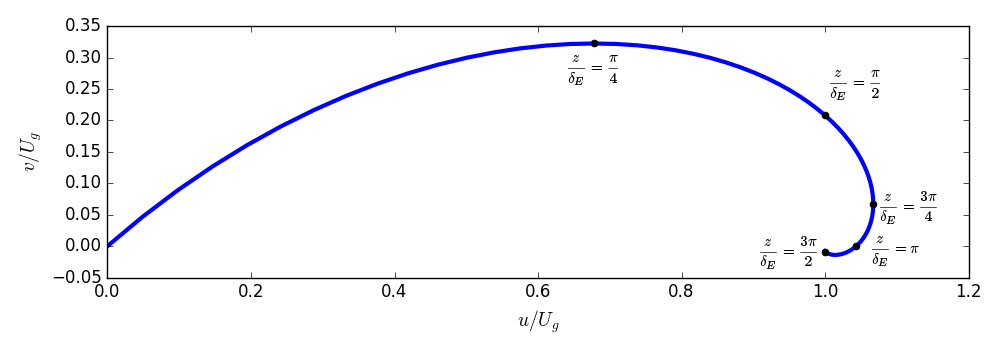
\includegraphics[width=\textwidth]{ekman2.png}	
	\end{figure}
\end{frame}
%------------------------------------------------
\begin{frame}{The Ekman Layer: Vertical Profiles}

Vertical profiles
	\begin{figure}
		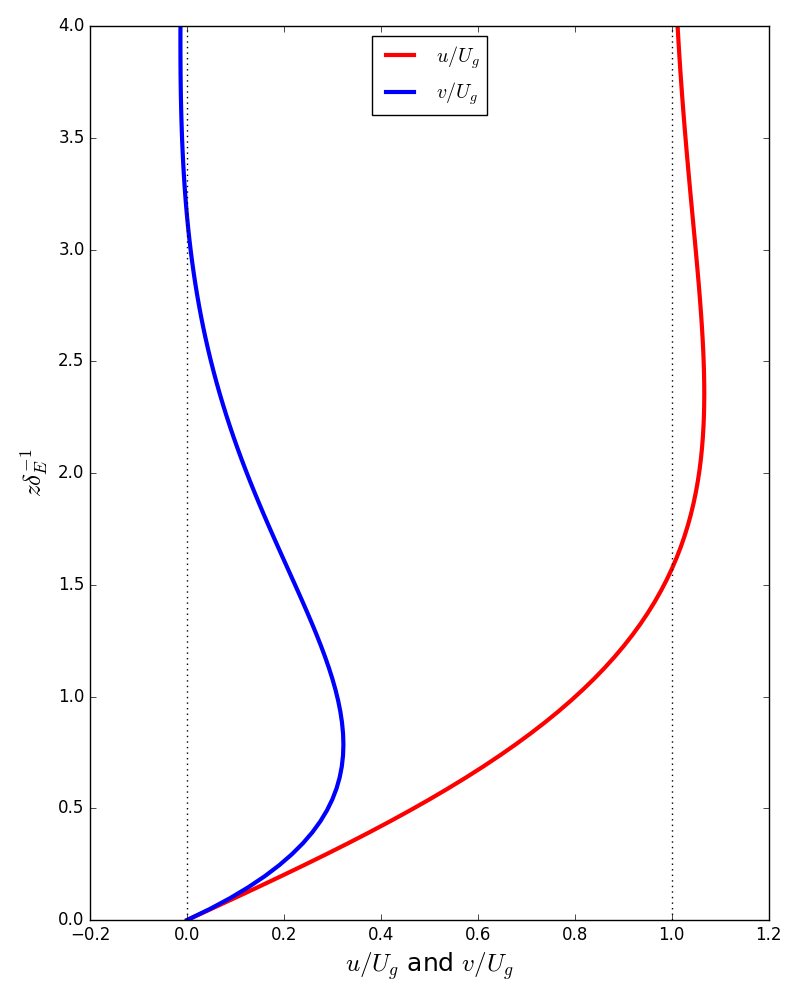
\includegraphics[width=0.55\textwidth]{ekman3.png}	
	\end{figure}
\end{frame}
%------------------------------------------------
\subsection{Flow Characteristics}
\begin{frame}{The Ekman Layer: Ekman Flow}

\begin{itemize}
	\item From the Ekman solution we see that friction induces a flow component directed toward low pressure.
	\item Ekman Depth $\delta_E$ is the measure of frictional boundary layer thickness.
	\item At $z=\delta_E$, the wind is approximately 80\% geostrophic.
	\item $\delta_E = \sqrt{2\nu/f}$
	\begin{itemize}
	\item As friction increases, the thickness increases
	\item As Coriolis increases, the thickness decreases
	\end{itemize}
\end{itemize}
\end{frame}
%------------------------------------------------
\begin{frame}{The Ekman Layer: Ekman Flow}

\begin{itemize}
	\item The observed Ekman depths in the atmosphere are on the order of $1000\ \metre$.
	\item Theory says:
	$$\delta_E = \sqrt{\frac{2\nu}{f}} = \sqrt{\frac{2\times 1.4 \times 10^{-5}\ \metre\squared\ \reciprocal\second}{10^{-4}\ \reciprocal\second}} \sim -0.5\ \metre$$
	\item Those ... are ... not close! Why?
	\item The atmosphere is turbulent, so $\vv{U} = \vv{U}(x,y,z,t)$ and not $\vv{U}=\vv{U}(z)$.
	\item However, if we take the spatial average of the Navier Stokes equations, the averaged equations look like the un-averaged equations but with molecular viscosity $\nu$ replaced with a much larger eddy-viscosity $\nu_E$.
\end{itemize}
\end{frame}

%------------------------------------------------
\begin{frame}{The Ekman Layer: Ekman Flow}

\begin{itemize}
	\item We can compute the eddy-viscosity based on the observed Ekman depth:
	$$\sqrt{\frac{2\nu_E}{f}} = 1000\ \metre \rightarrow \nu_E = \frac{f}{2}(1000\ \metre)^2 \sim 50\ \metre\squared\ \reciprocal\second$$
	\item True Ekman spirals do not exist in nature.
	\item However, modified (flatter) spirals are observed, as well as the theoretical result that low-level flow cuts across isobars toward low-pressure.
	\item If streamlines are curved, Ekman theory is not strictly valid  because $u$ and $v$ vary in $x$ and $y$, respectively, as well as in $z$ (but it's approximately valid).
	\item We will apply Ekman concepts locally by assuming that the velocity profile at a local point behaves like an Ekman velocity profile.
\end{itemize}
\end{frame}
%------------------------------------------------
\subsection{Ekman Pumping}
\begin{frame}{The Ekman Layer: Ekman Pumping}

\begin{itemize}
	\item The horizontal pressure gradient aloft is largely present at low levels. 
	\item At low levels, friction induces a flow component toward low pressure. 
	\item As a result, we get horizontal convergence into the low-pressure zone.
	\item This results in rising motion (from mass conservation).
	\item This can lead to condensation, rain, clouds, storms, etc.
	\begin{figure}
	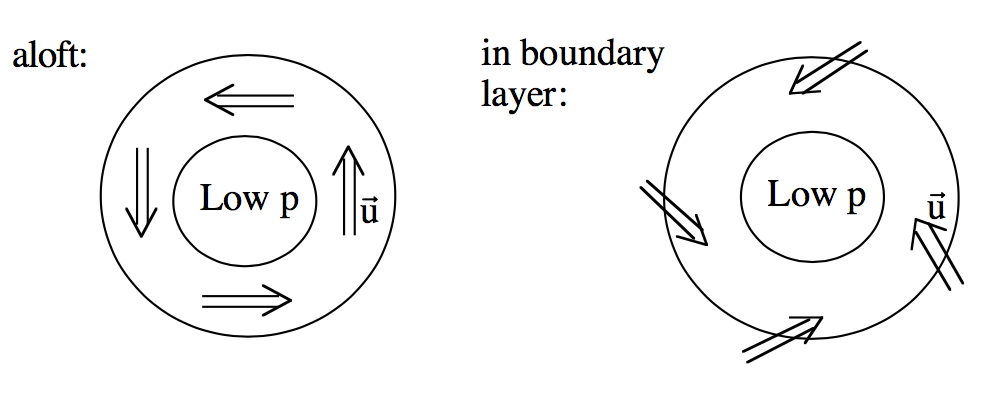
\includegraphics[width=0.7\textwidth]{ekman4}	
	\end{figure}
\end{itemize}
\end{frame}
%------------------------------------------------
\end{document}

